\documentclass[tikz,border=10pt]{standalone}
\usetikzlibrary{calc}
\begin{document}
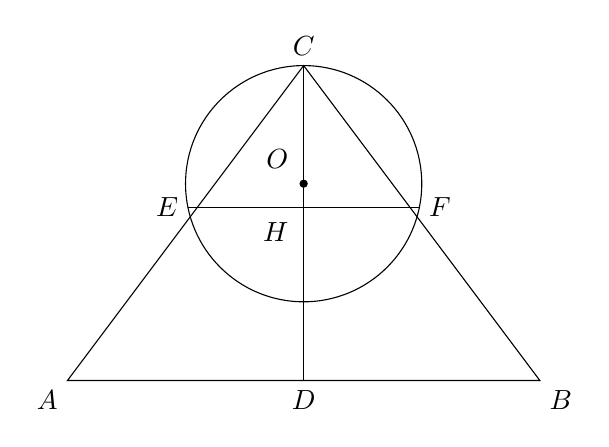
\begin{tikzpicture}[scale=1]
  \coordinate (A) at (-3,0);
  \coordinate (B) at (3,0);
  \coordinate (C) at (0,4);
  \coordinate (D) at (0,0);
  \coordinate (O) at (0,2.5);
  \coordinate (H) at (0,2.2);
  \coordinate (E) at (-1.47,2.2);
  \coordinate (F) at (1.47,2.2);

  \draw (A) -- (B) -- (C) -- cycle;
  \draw (C) -- (D);
  \draw (E) -- (F);
  \draw (O) circle (1.5);
  \fill (O) circle (1.5pt);

  \node[below left] at (A) {$A$};
  \node[below right] at (B) {$B$};
  \node[above] at (C) {$C$};
  \node[below] at (D) {$D$};
  \node[above left=2pt] at (O) {$O$};
  \node[below left=2pt] at (H) {$H$};
  \node[left] at (E) {$E$};
  \node[right] at (F) {$F$};
\end{tikzpicture}
\end{document}
